\section{Phase 2: Runtime Optimization Under Expected Conditions}
\label{phase2}

\subsection{Goal}
Experiments in this phase seek to tease out relationships between properties of the input data and runtime. Runtime on its own is a rather coarse measurement. For our \aspop{} solver, there are two logical means of fragmenting runtime into its principal components:

\begin{enumerate}
\item per \gls{suffix filter} block length

Patterns perform several \glspl{query} to the \gls{text index}, each with a different length of \gls{filter}. Aggregating like-sized filters will allow us a view into how filters of different lengths share the load of solving the problem, and identify algorithmic bottlenecks related to filters of only certain lengths.

\item per \gls{filter algorithm} step

The \gls{search step}'s runtime is a function of the shape of the query-search trees for each \gls{pattern}, which is in turn a function just about everything. The verification time is dependent on the number of \glspl{candidate} from the search step, as well as the rate at which candidates are \textit{spurious}.
\end{enumerate}

Very many properties can be extracted from a data set and reasoned over. Identifying the implications of properties that are \textit{intuitive} provides insight into what is actually happening inside the solver. Four such properties were identified and tested:

\begin{enumerate}
\item Genome Length

The length of the \gls{source genome} mostly affects the number of \glspl{read} in the data set without greatly\footnote{The impact of genome length on runtime is small when compared to a comparable increase in coverage, the most similar data set property. This is because both properties increase the number of reads to the same degree, but coverage usually introduces highly \textit{similar} reads leading to more text index hits and more overlap solutions.} impacting the number of overlaps per read. More reads also mean a longer \gls{text}, which has the side effect of more text index `hits', reducing pruning in query search trees. Unless otherwise specified, genome length is kept consistently at around 9600 nucleotides.

\item Read Length

Read length controls the \textit{maximum} length of a read (some fragments end up shorter). Read length is determined \textit{independently} to source genome length and \gls{coverage}; As the read length increases, the number of reads in the data set decreases. This is truly a measure of the \textit{fragmentation} of the source genome, not to be confused with coverage. Except in this experiment where it is the response variable, read length is consistently kept at approximately 250bp  (base pairs).

\item Coverage

Coverage is a measure of the number of \glspl{genome copy} composing the data set\footnote{Coverage has different specific definitions depending on the source. See the glossary definition of `coverage' for details. For our purpose, it is sufficient to consider coverage to be uniform across the length of the genome, being analogous to the count of genome copies in the data set.}. With a higher-coverage data set, there are more reads and more overlaps (in the \gls{search step} as well as the resulting \gls{solution} set). When not otherwise specified, experimental data sets have 500x coverage.

\item Divergence

If reads in a dataset are drawn from more than one source genome, one can reason about these genomes' divergence with respect to one another. Genomes with low divergence have a lot in common, and will contain more of the same substrings; A data set built from low-divergence genomes will likely result in more overlaps being found. For the coverage and divergence experiments, the data is drawn from real sources, with unknown constant values of coverage. For the other two experiments divergence is not defined, as only one source genome was used.

\end{enumerate}

\subsection{Experimental Design}
A battery of four experiment \textit{groups} tested the same target variables, but each time in response to a different \textit{data set property}. For each group, two experiments were performed:

\begin{enumerate}
\item Total runtimes (along with runtimes fragmented per \gls{filter algorithm} step) shown according to the given predictor variable.

\item Proportion of total runtime distributed across different \gls{filter} lengths, plotted across values of the predictor variable.
\end{enumerate}

% \FloatBarrier
\subsection{Results}
Figures \ref{fig:gnmlen} - \ref{fig:div} show the effect the various properties of the data set had on the runtime, as seen in two different partitions: per \gls{filter algorithm} step and per \gls{filter} blocks.



\begin{figure}
\centering
\makebox[\linewidth][c]{%
\begin{subfigure}[t]{.53\textwidth}
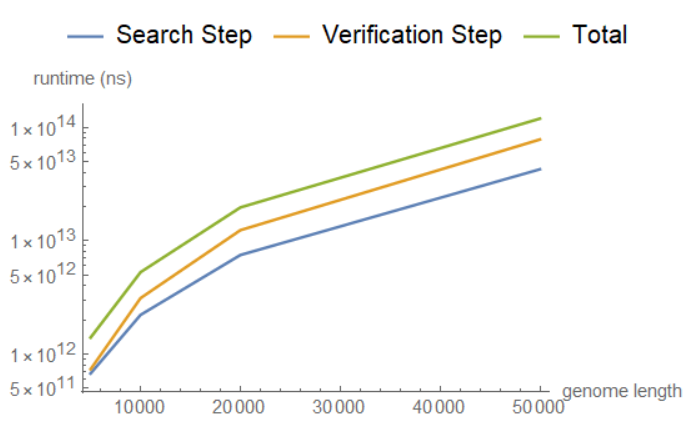
\includegraphics[width=1\linewidth]{images/gnmlen_a.png}
\caption{}
\end{subfigure}
~
\begin{subfigure}[t]{.53\textwidth}
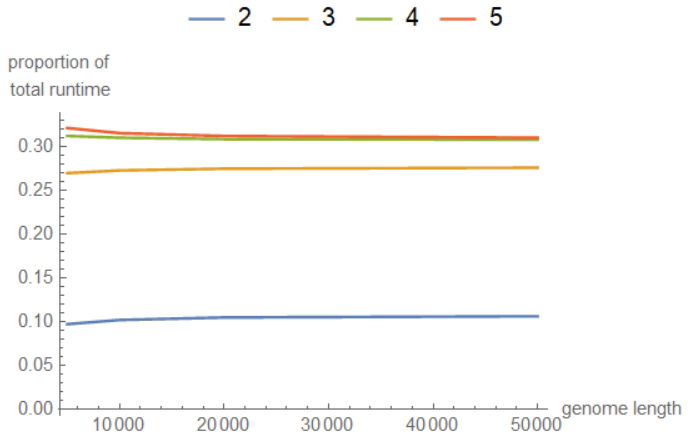
\includegraphics[width=1\linewidth]{images/gnmlen_b.png}
\caption{}
\end{subfigure}
}
\caption[Work time of \aspop{} solver runs partitioned into principal components, plotted as a function of \textit{genome length}]{Work of \aspop{} solver runs partitioned into principal components, plotted as a function of \textit{genome length}.\\(a) Total runtime (in nanoseconds) partitioned by filter algorithm step.\\(b) Runtime proportion partitioned by suffix filter block lengths.}
\label{fig:gnmlen}
\end{figure}



\begin{figure}
\centering
\makebox[\linewidth][c]{%
\begin{subfigure}[t]{.53\textwidth}
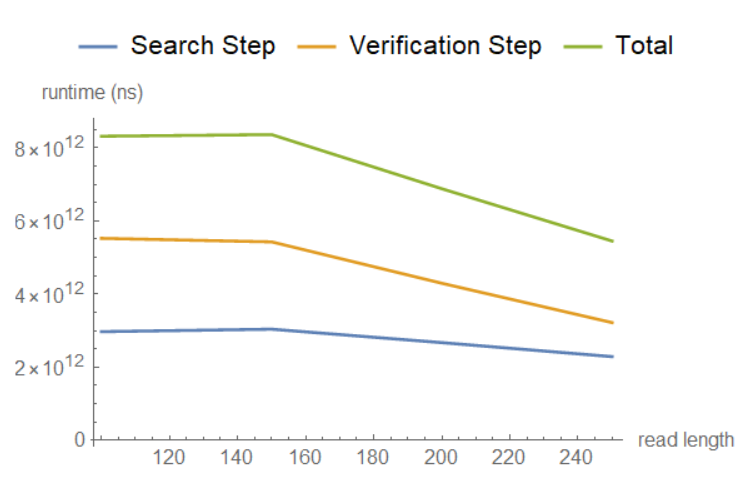
\includegraphics[width=1\linewidth]{images/rdlen_a.png}
\caption{}
\end{subfigure}
~
\begin{subfigure}[t]{.53\textwidth}
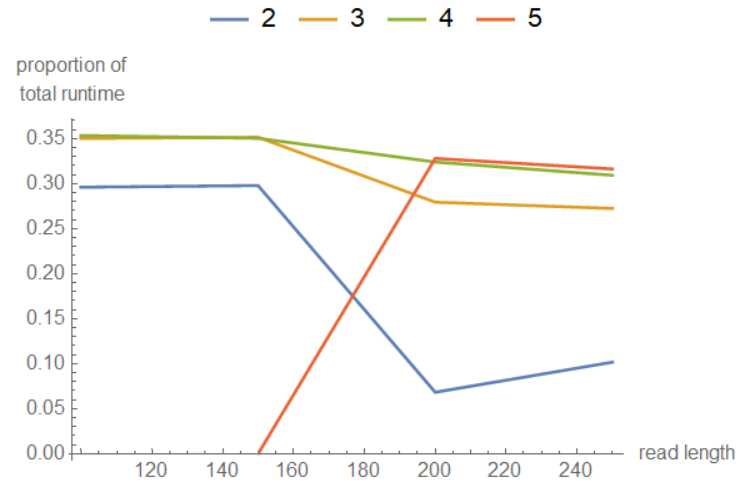
\includegraphics[width=1\linewidth]{images/rdlen_b.png}
\caption{}
\end{subfigure}
}
\caption[Work time of \aspop{} solver runs partitioned into principal components, plotted as a function of \textit{read length}]{Work of \aspop{} solver runs partitioned into principal components, plotted as a function of \textit{read length}.\\(a) Total runtime (in nanoseconds) partitioned by filter algorithm step.\\(b) Runtime proportion partitioned by suffix filter block lengths.}
\label{fig:rdlen}
\end{figure}



\begin{figure}
\centering
\makebox[\linewidth][c]{%
\begin{subfigure}[t]{.53\textwidth}
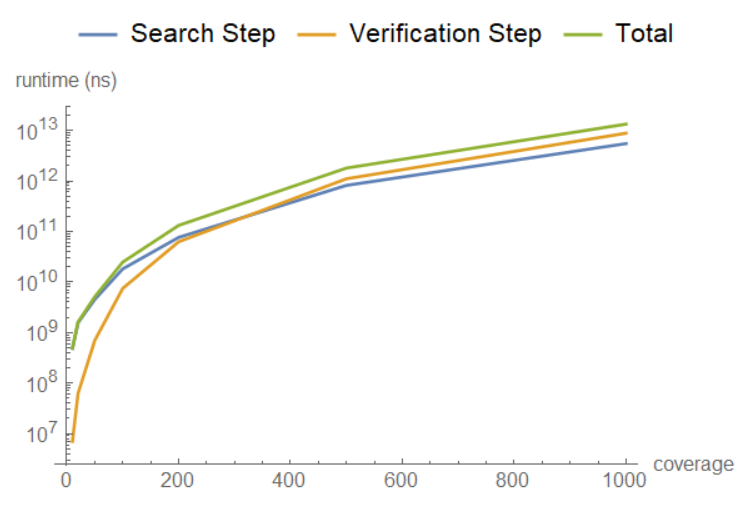
\includegraphics[width=1\linewidth]{images/cov_a.png}
\caption{}
\end{subfigure}
~
\begin{subfigure}[t]{.53\textwidth}
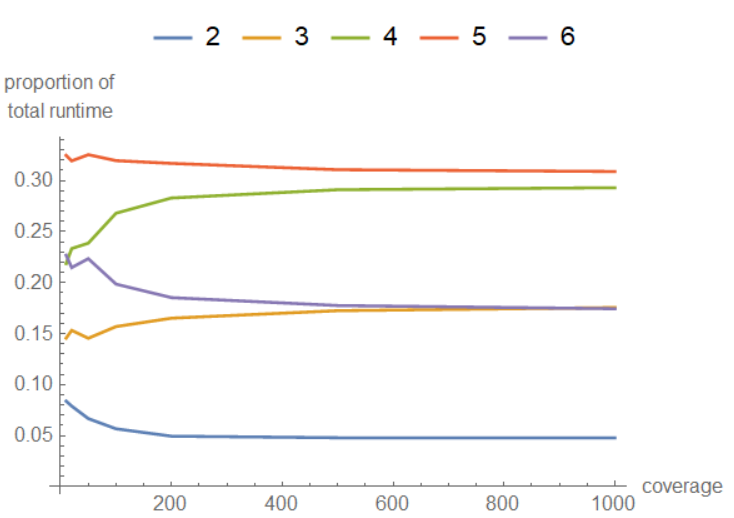
\includegraphics[width=1\linewidth]{images/cov_b.png}
\caption{}
\end{subfigure}
}
\caption[Work time of \aspop{} solver runs partitioned into principal components, plotted as a function of \textit{genome coverage}]{Work of \aspop{} solver runs partitioned into principal components, plotted as a function of \textit{genome coverage}.\\(a) Total runtime (in nanoseconds) partitioned by filter algorithm step.\\(b) Runtime proportion partitioned by suffix filter block lengths.}
\label{fig:cov}
\end{figure}



\begin{figure}
\centering
\makebox[\linewidth][c]{%
\begin{subfigure}[t]{.53\textwidth}
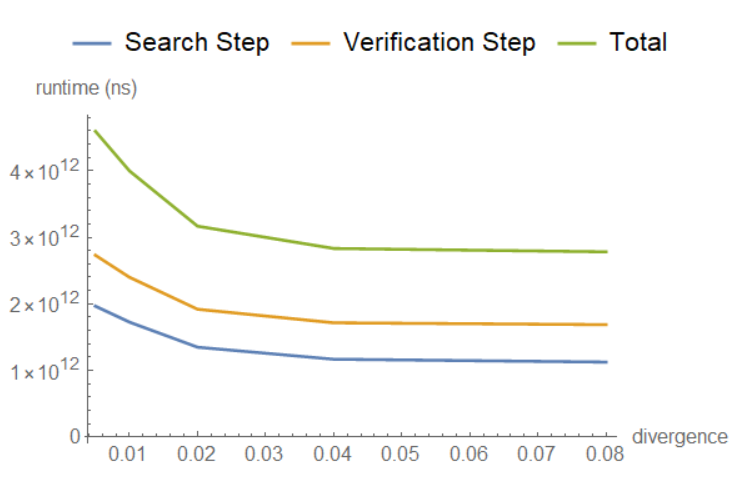
\includegraphics[width=1\linewidth]{images/div_a.png}
\caption{}
\end{subfigure}
~
\begin{subfigure}[t]{.53\textwidth}
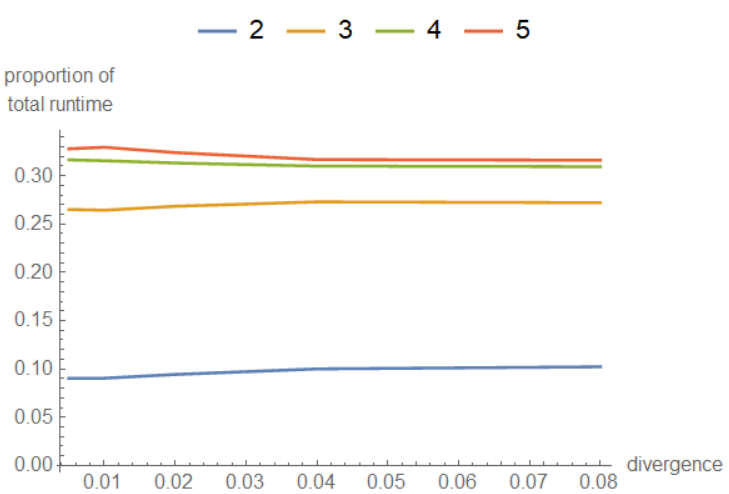
\includegraphics[width=1\linewidth]{images/div_b.png}
\caption{}
\end{subfigure}
}
\caption[Work time of \aspop{} solver runs partitioned into principal components, plotted as a function of \textit{genome divergence}]{Work of \aspop{} solver runs partitioned into principal components, plotted as a function of \textit{genome divergence}.\\(a) Total runtime (in nanoseconds) partitioned by filter algorithm step.\\(b) Runtime proportion partitioned by suffix filter block lengths.}
\label{fig:div}
\end{figure}

\FloatBarrier

\subsection{Observations}

Increased \textit{read length} in fig \ref{fig:rdlen} (a) demonstrated that for the same amount of data overall, the algorithm \textit{sped up} when faced with a smaller number of longer \glspl{read}, but not to an extreme extent. From (b), one can observe the longer \glspl{filter} beginning to `kick in' only for longer read lengths, as would be expected. It is notable here that filters took time roughly correspondent to their length. This is desirable behavior as it indicates that the workload is evenly distributed amongst filters (as much as their varying lengths will allow) and that no obvious niche cases are causing overwhelming slowdown. 
\begin{figure}[]
\centering
\makebox[\linewidth][c]{%
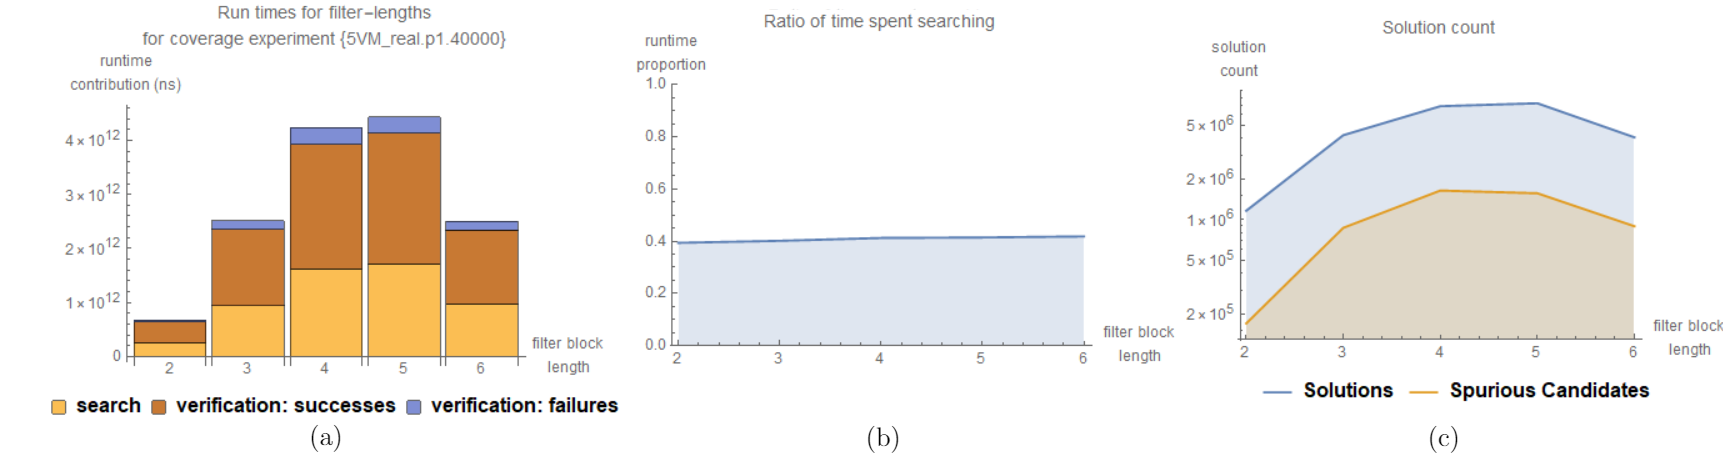
\includegraphics[width=1.3\textwidth]{images/cov40k_details.png}
}
\caption[Details of runtime for run `dataset\_coverage\_1000x'.]{Details of runtime for run `dataset\_coverage\_1000x'.\\(a) Runtime contributions for steps of the filter algorithm.\\(b) Ratio of time spent searching per filter block length.\\(c) Solution counts that did and did not verify per filter block length.}
\label{fig:cov40k_details}
\end{figure}
Increased \gls{coverage} proportionately increases the size of a data set, but increases the size of the \gls{solution} set super-linearly. As such, it is interesting to observe in Figure \ref{fig:cov} (a) that both steps of the \gls{filter algorithm} do not increase in lockstep, but the \gls{verification step} overtakes the \gls{search step} in runtime for high-coverage data. This was also visible in Figure \ref{fig:gnmlen} (a). Figure \ref{fig:cov} (b) Shows a trend for medium-length filters to contribute more to run time; Figure \ref{fig:cov40k_details} observes this in more detail, and shows that it is justified, with filters consistently spending more time working when they find more \glspl{solution}. Longest filters are shown to find fewer solutions than medium-length filters; This could be due to patterns differing in lengths and, consequently, several patterns simply not having a 6th filter to contribute to the overall runtime and solution set. The stabilizing proportions in Figure \ref{fig:cov} (b) are best explained as the law of large numbers at work; With low coverage (a smaller read set), the work contribution proportions are rather unstable. Why exactly these proportions seem to gravitate to fixed positions in a continuous direction and not in a zig-zagging fashion is unknown.




Increased \textit{divergence} in Figure \ref{fig:div} (a) was marked with a consistent reduction in overall runtime. This is to be expected as the data set's \glspl{source genome} have fewer overlaps in common, causing a more spindly search tree in the \gls{search step} as \glspl{match location} dry up. The  behavior of the individual filters remained relatively consistent for filters across the values of divergence. Figure \ref{fig:div} (b) shows that the distribution of work remains remarkably stable, maintaining the predicted relative positions across different solver executions.

\FloatBarrier